\documentclass[14pt,a4paper,report]{report}
\usepackage[a4paper, mag=1000, left=2.5cm, right=1cm, top=2cm, bottom=2cm, headsep=0.7cm, footskip=1cm]{geometry}
\usepackage[utf8]{inputenc}
\usepackage[english,russian]{babel}
\usepackage{indentfirst}
\usepackage[dvipsnames]{xcolor}
\usepackage[colorlinks]{hyperref}
\usepackage{listings} 
\usepackage{fancyhdr}
\usepackage{caption}
\usepackage{graphicx}
\hypersetup{
	colorlinks = true,
	linkcolor  = black
}

\usepackage{titlesec}
\titleformat{\chapter}
{\Large\bfseries} % format
{}                % label
{0pt}             % sep
{\huge}           % before-code


\DeclareCaptionFont{white}{\color{white}} 

% Listing description
\usepackage{listings} 
\DeclareCaptionFormat{listing}{\colorbox{gray}{\parbox{\textwidth}{#1#2#3}}}
\captionsetup[lstlisting]{format=listing,labelfont=white,textfont=white}
\lstset{ 
	% Listing settings
	inputencoding = utf8,			
	extendedchars = \true, 
	keepspaces = true, 			  	 % Поддержка кириллицы и пробелов в комментариях
	language = C,            	 	 % Язык программирования (для подсветки)
	basicstyle = \small\sffamily, 	 % Размер и начертание шрифта для подсветки кода
	numbers = left,               	 % Где поставить нумерацию строк (слева\справа)
	numberstyle = \tiny,          	 % Размер шрифта для номеров строк
	stepnumber = 1,               	 % Размер шага между двумя номерами строк
	numbersep = 5pt,              	 % Как далеко отстоят номера строк от подсвечиваемого кода
	backgroundcolor = \color{white}, % Цвет фона подсветки - используем \usepackage{color}
	showspaces = false,           	 % Показывать или нет пробелы специальными отступами
	showstringspaces = false,    	 % Показывать или нет пробелы в строках
	showtabs = false,           	 % Показывать или нет табуляцию в строках
	frame = single,              	 % Рисовать рамку вокруг кода
	tabsize = 2,                  	 % Размер табуляции по умолчанию равен 2 пробелам
	captionpos = t,             	 % Позиция заголовка вверху [t] или внизу [b] 
	breaklines = true,           	 % Автоматически переносить строки (да\нет)
	breakatwhitespace = false,   	 % Переносить строки только если есть пробел
	escapeinside = {\%*}{*)}      	 % Если нужно добавить комментарии в коде
}

\begin{document}

\def\contentsname{Содержание}

% Titlepage
\begin{titlepage}
	\begin{center}
		\textsc{Санкт-Петербургский Политехнический 
			Университет Петра Великого\\[5mm]
			Кафедра компьютерных систем и программных технологий}
		
		\vfill
		
		\textbf{Отчёт по лабораторной работе №1\\[3mm]
			Курс: «Защита информации»\\[6mm]
			Тема: «Исследование сетевого трафика»\\[35mm]
		}
	\end{center}
	
	\hfill
	\begin{minipage}{.5\textwidth}
		Выполнил студент:\\[2mm] 
		Бояркин Никита Сергеевич\\
		Группа: 43501/3\\[5mm]
		
		Проверил:\\[2mm] 
		Новопашенный Андрей Гелиевич
	\end{minipage}
	\vfill
	\begin{center}
		Санкт-Петербург\\ \the\year\ г.
	\end{center}
\end{titlepage}

% Contents
\tableofcontents
\clearpage

\chapter{Лабораторная работа №1}

\section{Цель работы}

Получение навыков по исследованию сетевого трафика.

\section{Программа работы}

При помощи программы WireShark продемонстрировать сетевой трафик для:

\begin{itemize}
	\item Утилиты ping
		\begin{itemize}
			\item Без фрагментации
			\item С фрагментацией
		\end{itemize}
	\item Утилиты tracert
	\item Протокола ICMP
	\item Протокола ARP
		\begin{itemize}
			\item Запрос
			\item Ответ
		\end{itemize}
	\item Протокола TCP
		\begin{itemize}
			\item Установление соединения
			\item Разрыв соединения
			\item Попытка соединения на отсутствующий порт
		\end{itemize}
\end{itemize}

\section{Конфигурация сети}

\begin{figure}[h!]
	\centering
	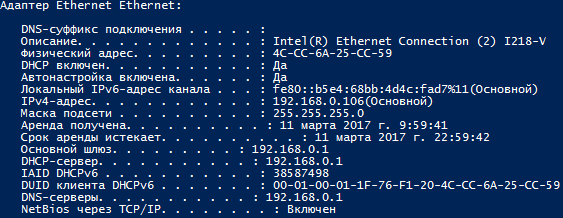
\includegraphics[scale = 1.1]{images/config.png}
	
	\caption{Сетевые параметры компьютера}
	\label{image:1}
\end{figure}

\clearpage

\section{Ход работы}

\subsection{Утилита Ping}

Утилита Ping отправляет эхо-запрос ICMP, после чего, в случае успеха должен прийти симметричный эхо-ответ ICMP. Если пакет не пришел за некоторое время, то удаленный сервер считается недостижимым. По умолчанию производится четыре попытки.

\subsubsection{Ping без фрагментации}

Трафик утилиты Ping со стандартными параметрами ($bytes=128, TTL=128$):

\begin{figure}[h!]
	\centering
	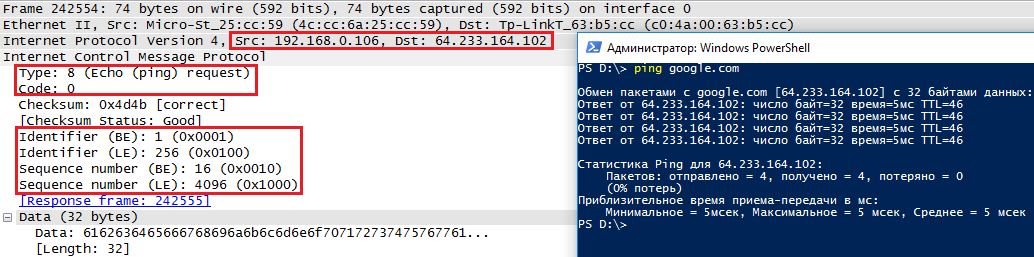
\includegraphics[scale = 0.65]{images/ping1.png}
	
	\caption{ICMP эхо-запрос}
	\label{image:2}
\end{figure}

\begin{figure}[h!]
	\centering
	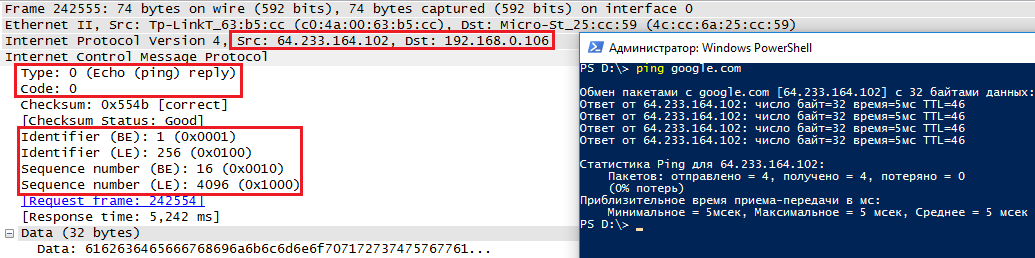
\includegraphics[scale = 0.65]{images/ping2.png}
	
	\caption{ICMP эхо-ответ}
	\label{image:3}
\end{figure}

Пакеты были распознаны как ICMP с пометкой "Echo (ping) reply/request", что означает эхо запрос/ответ. Графа Destination показывает IP адрес удаленного сервера, который мы пингуем, Source показывает IP адрес текущего компьютера.

Поля "Identifier" и "Sequence number" присутствуют только в эхо запросе/ответе (ICMP типы 0 и 8) и необходимы для сопоставления ответа и запроса.

\clearpage

\subsubsection{Ping с фрагментацией}

Для фрагментации пакета необходимо явно указать его размер, превышающий MTU (maximum transmission unit) - максимальный размер полезного блока данных одного пакета, который может быть передан без фрагментации. Для интерфейса Ethernet II значение MTU равно 1500 байт. Тогда без учета заголовка (20 байт) длина одного фрагмента не превышает 1480 байт.

Трафик утилиты Ping с измененными параметрами ($bytes=4096, TTL=61$):

\begin{figure}[h!]
	\centering
	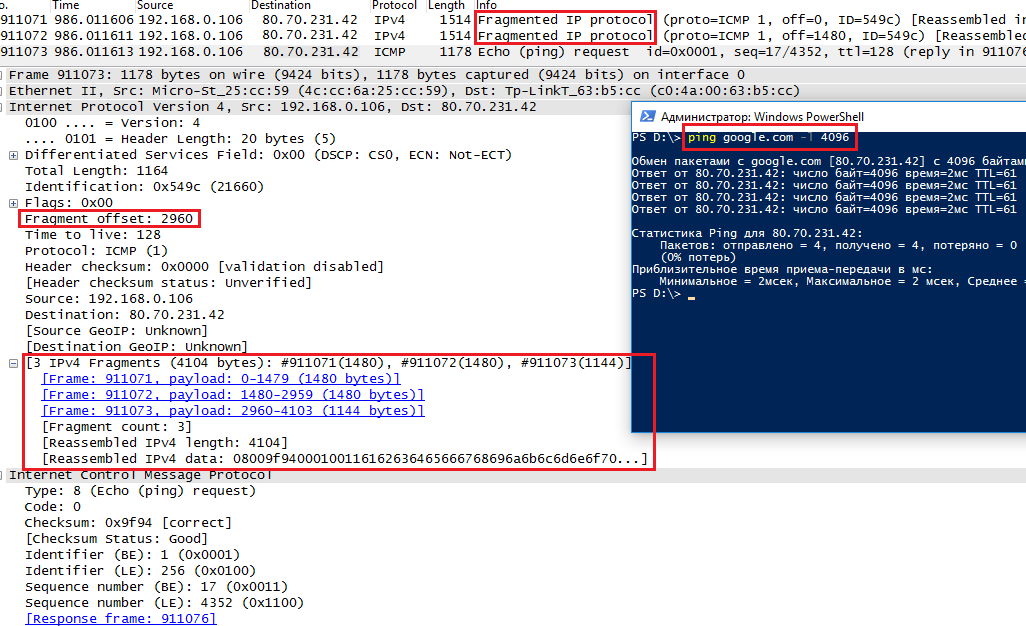
\includegraphics[scale = 0.66]{images/ping3.png}
	
	\caption{Фрагментированный эхо-запрос (последний фрагмент)}
	\label{image:4}
\end{figure}

Видно, что пакет разделился на три части. Стоит отметить, что фрагментация пакета осуществляется на уровне IP и каждый фрагмент имеет одинаковое значение поля "Identificaton". 

\begin{figure}[h!]
	\centering
	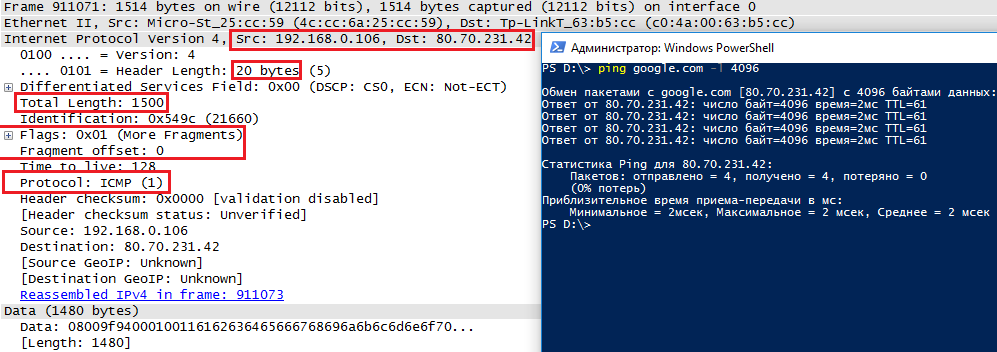
\includegraphics[scale = 0.67]{images/ping4.png}
	
	\caption{Фрагментированный эхо-запрос (первый фрагмент)}
	\label{image:5}
\end{figure}

Флаги, установленные в 0x1 свидетельствуют о наличии других фрагментов. Первый фрагмент определяется нулевым смещением.

\subsection{Утилита Tracert}

Tracert базируется на использовании поля TTL протокола ICMP. Первый пакет имеет TTL=1, для каждого последующего пакета TTL инкрементируется. Это продолжается до тех пор пока не придет эхо-ответ, а не ошибка истечения TTL. Трафик tracert это набор ICMP пакетов с типом "Time-to-live exceeded" (код 0x11) и в случае успеха, последний успешный эхо-ответ.

\begin{figure}[h!]
	\centering
	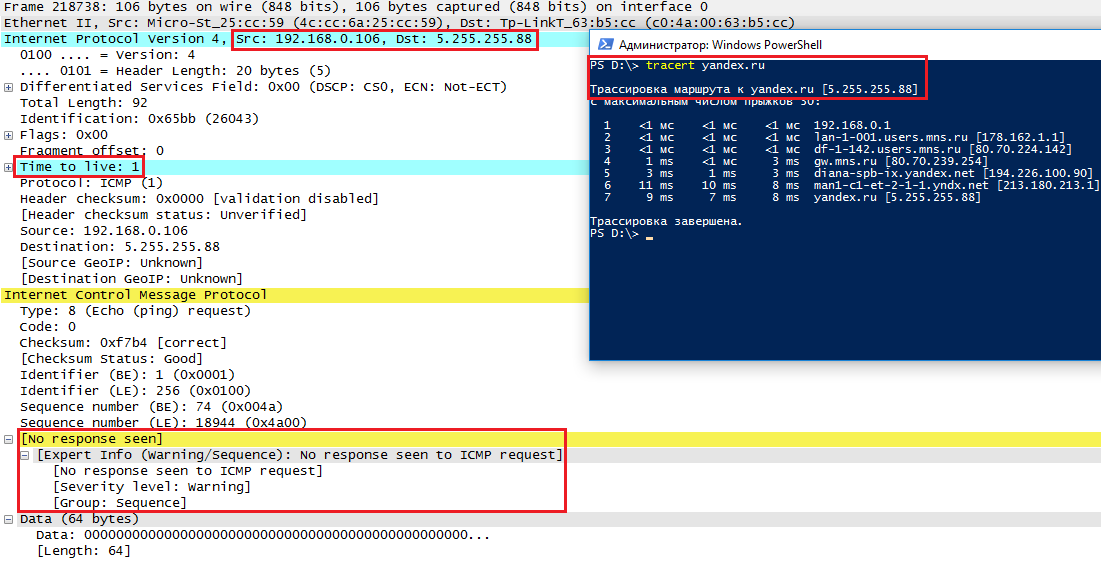
\includegraphics[scale = 0.62]{images/tracert1.png}
	
	\caption{Процесс трассировки yandex.ru (первый ICMP эхо-запрос)}
	\label{image:6}
\end{figure}

Видно, что первый эхо-запрос имеет TTL равный единице, это означает, что на первом же маршрутизаторе, проверяющем значение TTL пакет будет уничтожен и вернется сообщение об ошибке.

\begin{figure}[h!]
	\centering
	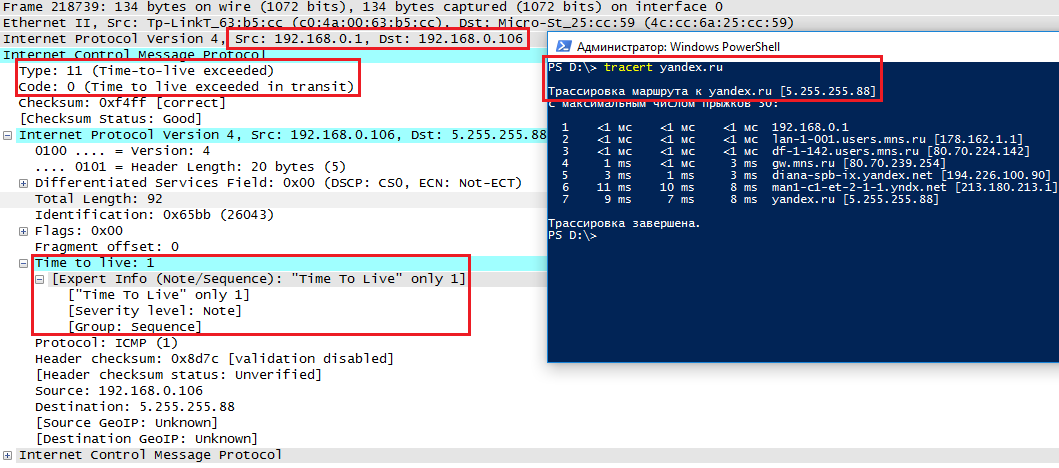
\includegraphics[scale = 0.62]{images/tracert2.png}
	
	\caption{Процесс трассировки yandex.ru (сообщение об ошибке Time-to-live exceeded)}
	\label{image:7}
\end{figure}

Как и ожидалось, первая остановка это сетевой шлюз. В этом узле TTL стало равным нулю и был отправлен ICMP пакет с ошибкой типа "Time-to-live exceeded".

\clearpage

\subsection{Протокол ICMP}

ICMP ошибка о недоступности хоста (host unreachable) отправляется маршрутизатором, когда он получает IP датаграмму, которую невозможно перенаправить. Для получения данной ошибки в домашней сети будем пинговать тот локальный IP адрес, к которому шлюз по умолчанию не сможет проложить маршрут. 

\begin{figure}[h!]
	\centering
	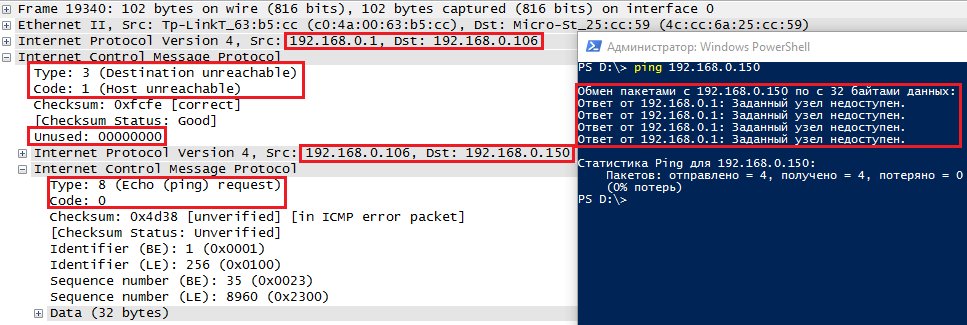
\includegraphics[scale = 0.69]{images/icmp1.png}
	
	\caption{ICMP ошибки недоступности адресата}
	\label{image:8}
\end{figure}

В результате, на каждый посылаемый ICMP эхо запрос, вернулись ICMP пакеты с ошибкой "Dectination unreacheble (Host unreacheable)" с типом 0x3 и кодом 0x1. Особенностью данной ошибки является то, что она посылается от шлюза, а не от узла назначения, что не удивительно, потому что к нему не удалось проложить маршрут. Также, при данном типе ошибки присутствует 32-битное не используемое поле, исходный IP заголовок, а также первые 64-бита исходной дейтаграммы.

\begin{figure}[h!]
	\centering
	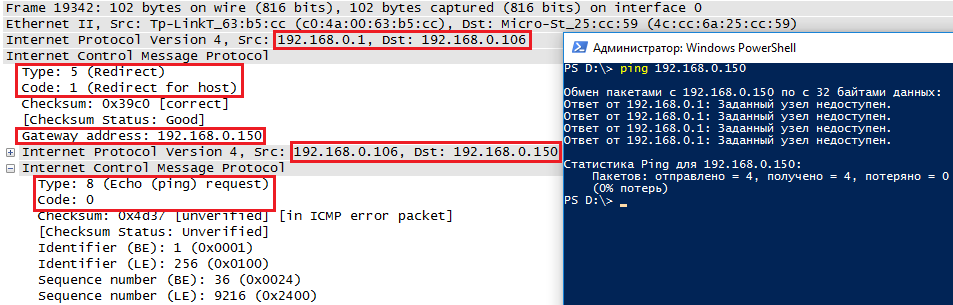
\includegraphics[scale = 0.69]{images/icmp2.png}
	
	\caption{ICMP информирование о перенаправлении}
	\label{image:9}
\end{figure}

После ICMP пакета "Dectination unreacheble (Host unreacheable)" следует ICMP пакет "Redirect (Redirect for host)", который информирует о том, что необходимо создать новый маршрут к указанному хосту и внести его в таблицу маршрутизации.

\clearpage

\subsection{Протокол ARP}

Рассмотрим пару APR пакетов, которая демонстрирует работу протокола.

\begin{figure}[h!]
	\centering
	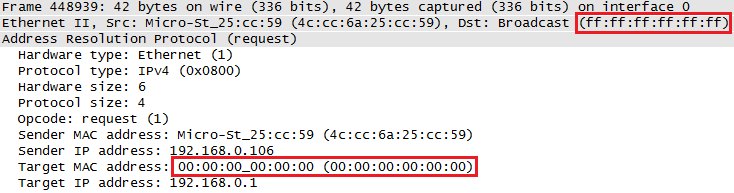
\includegraphics[scale =  0.85]{images/arp1.png}
	
	\caption{ARP запрос}
	\label{image:13}
\end{figure}

Был отправлен широковещательный ARP запрос с заданным полем "Target IP Address" и нулевым полем "Target MAC Address". 

\begin{figure}[h!]
	\centering
	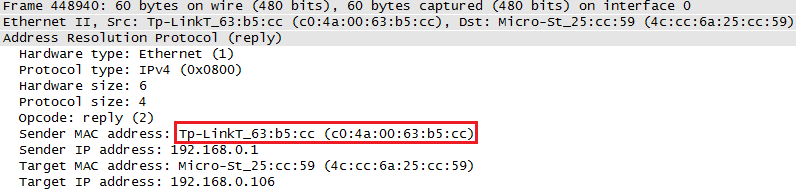
\includegraphics[scale = 0.80]{images/arp2.png}
	
	\caption{ARP ответ}
	\label{image:14}
\end{figure}

Был получен ARP ответ, в котором поле "Sender MAC Address" содержит искомый MAC адрес. Тип ARP пакета указывается в поле Opcode (запрос 0x1, ответ 0x2).

\subsection{Протокол TCP}

\subsubsection{Установление соединения}

Попробуем установить TCP соединение с помощью утилиты telnet.

\begin{figure}[h!]
	\centering
	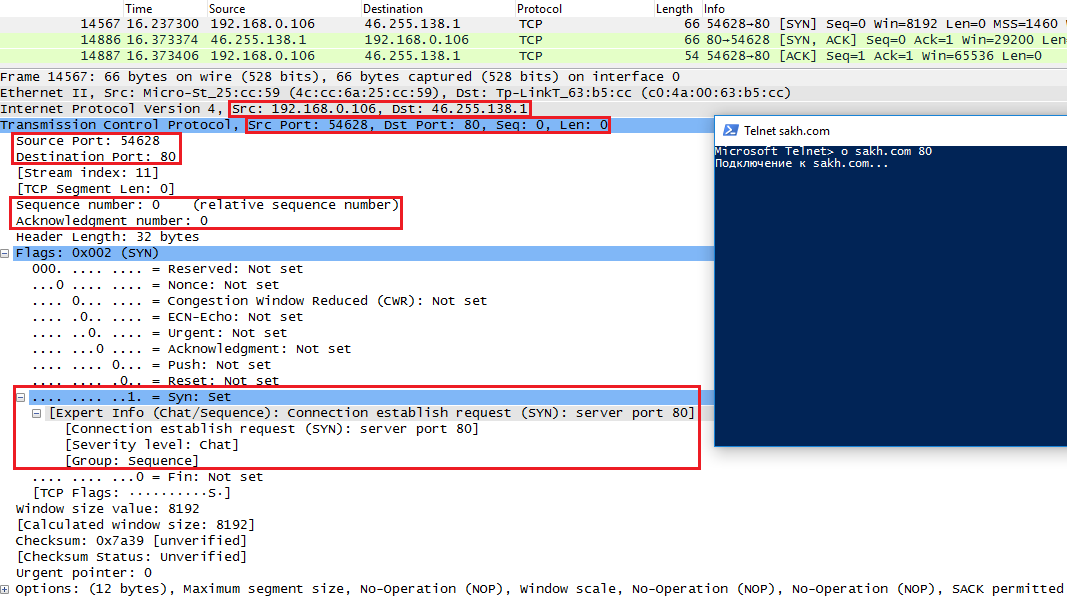
\includegraphics[scale = 0.63]{images/tcp1.png}
	
	\caption{TCP запрос на установление соединения SYN}
	\label{image:15}
\end{figure}

Для установления соединения посылается TCP пакет с управляющим битом SYN (синхронизация номеров последовательности) и номером последовательности. Сервер получает сегмент, запоминает номер последовательности и пытается создать сокет (буферы и управляющие структуры памяти) для обслуживания нового клиента. В случае успеха сервер посылает клиенту сегмент с номером последовательности и флагами SYN и ACK, и переходит в состояние SYN-RECEIVED. В случае неудачи сервер посылает клиенту сегмент с флагом RST.

В заголовке TCP пакета также присутствуют следующие поля:

\begin{itemize}
	\item \emph{Sequence Number} - Если установлен флаг SYN, то это изначальный порядковый номер — ISN (Initial Sequence Number), и первый байт данных, которые будут переданы в следующем пакете, будет иметь номер, равный ISN + 1. В противном случае, если SYN не установлен, первый байт данных, передаваемый в данном пакете, имеет этот порядковый номер.
	\item \emph{Acknowledgment Number} -  Если установлен бит ACK, то это поле содержит порядковый номер октета, который отправитель данного сегмента желает получить. Это означает, что все предыдущие октеты (с номерами от ISN+1 до ACK-1 включительно) были успешно получены.
\end{itemize}

В данном случае на сервер был отправлен пакет с флагом SYN и ISN=0. Был получен пакет с установленным флагом ACK и номером последовательности ACK=1, что означает, что пакет с ISN=0 был успешно получен. Также в этом пакете установлен флаг SYN и ISN=0, что означает, что ожидается ACK со стороны клиента. Последний пакет содержит только ACK=1 для сервера.

\begin{figure}[h!]
	\centering
	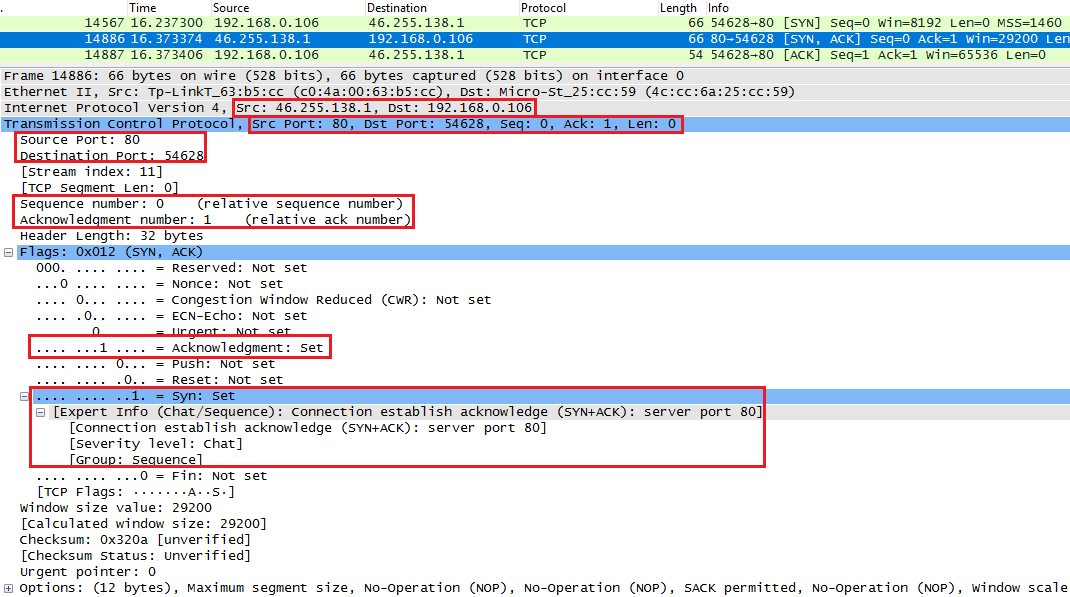
\includegraphics[scale = 0.62]{images/tcp2.png}
	
	\caption{Удачная установка TCP соединения (ответ с сервера)}
	\label{image:16}
\end{figure}

Ответ содержит установленные биты SYN и ACK, что свидетельствует об успешной установке соединения. 

\clearpage

\begin{figure}[h!]
	\centering
	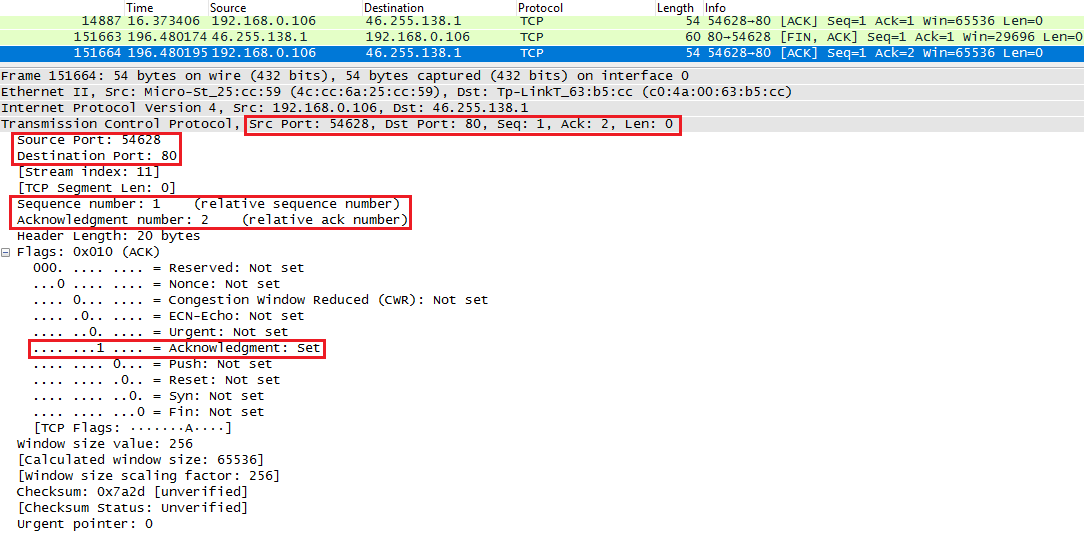
\includegraphics[scale = 0.61]{images/tcp3.png}
	
	\caption{Удачная установка TCP соединения (последний ACK)}
	\label{image:17}
\end{figure}

Последний этап это отправка на сервер пакета с установленным флагом ACK, после чего соединение переходит в состояние ESTABLISHED.

\subsubsection{Неудачное соединение}

Рассмотрим попытку неудачного соединения. Клиент посылает пакет с управляющим битом SYN (запрос на установление соединения рассмотрен в предыдущем пункте).

\begin{figure}[h!]
	\centering
	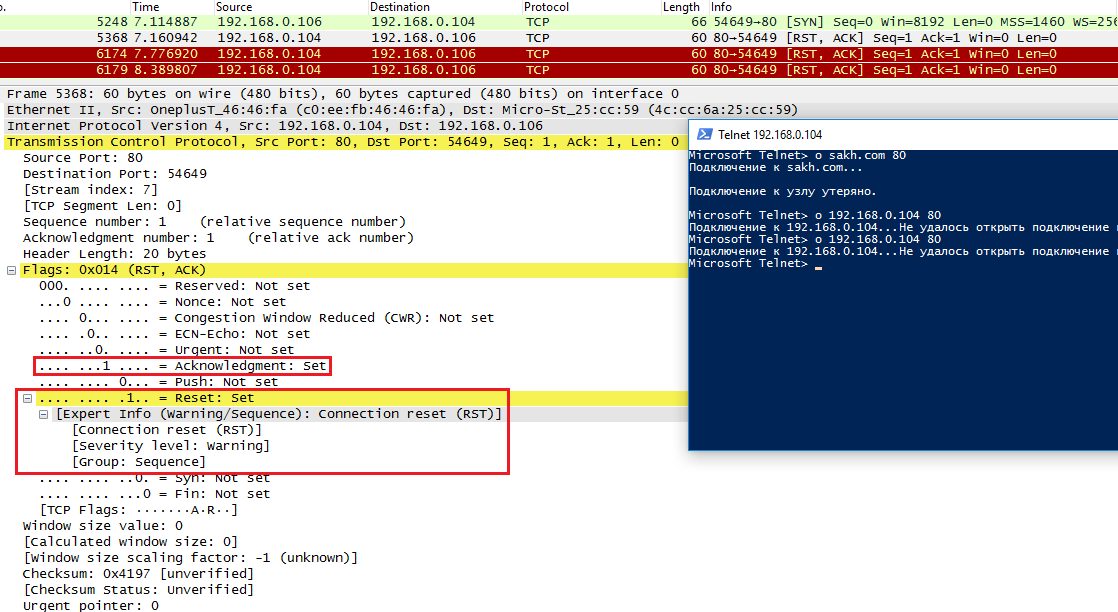
\includegraphics[scale = 0.60]{images/tcp4.png}
	
	\caption{Неудачная попытка TCP соединения}
	\label{image:18}
\end{figure}

Сервер посылает пакет с установленным управляющим битом RST. После чего клиент уже не пытается установить соединение.

\subsubsection{Завершение соединения}

Рассмотрим процесс завершения соединения (инициированного с серверной стороны):

\begin{figure}[h!]
	\centering
	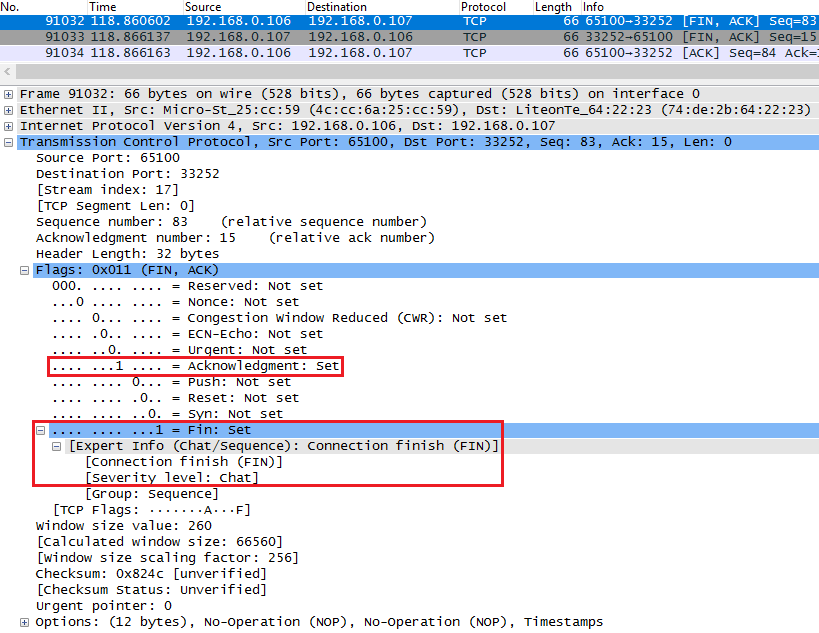
\includegraphics[scale = 0.70]{images/tcp5.png}
	
	\caption{Завершение TCP соединения}
	\label{image:19}
\end{figure}

Если соединение уже было установлено, то завершение соединения производится следующим образом:

\begin{itemize}
	\item Посылка серверу от клиента флага FIN на завершение соединения.
	\item Сервер посылает клиенту флаги ответа ACK , FIN, что соединение закрыто.
	\item После получения этих флагов клиент закрывает соединение и в подтверждение отправляет серверу ACK, что соединение закрыто.
\end{itemize}

В данном случае был запущен сервер по адресу 192.168.0.107:65100, после чего к нему подключился клиент. Клиент был принудительно отключен со стороны сервера: клиенту был отправлен пакет с установленными битами FIN и ACK, после чего клиент отправляет такой же пакет на сервер и переходит из состояния ESTABLISHED в состояние CLOSE WAIT, в завершении сервер отправляет клиенту ACK и переходит в состояние CLOSED, клиент получает ACK и также переходит в состояние CLOSED.

\clearpage

\subsubsection{Установка соединения с закрытым портом}

При попытке подключения к отсутствующему порту, не приходит ACK и RST, поэтому клиент находится в подвешенном состоянии и ожидает ответа. Такое поведение обусловлено работой межсетевого экрана, который не позволяет узнать извне какие порты открыты. Результат подключения к закрытому порту с отключенным межсетевым экраном рассмотрен в приложении 1.

\begin{figure}[h!]
	\centering
	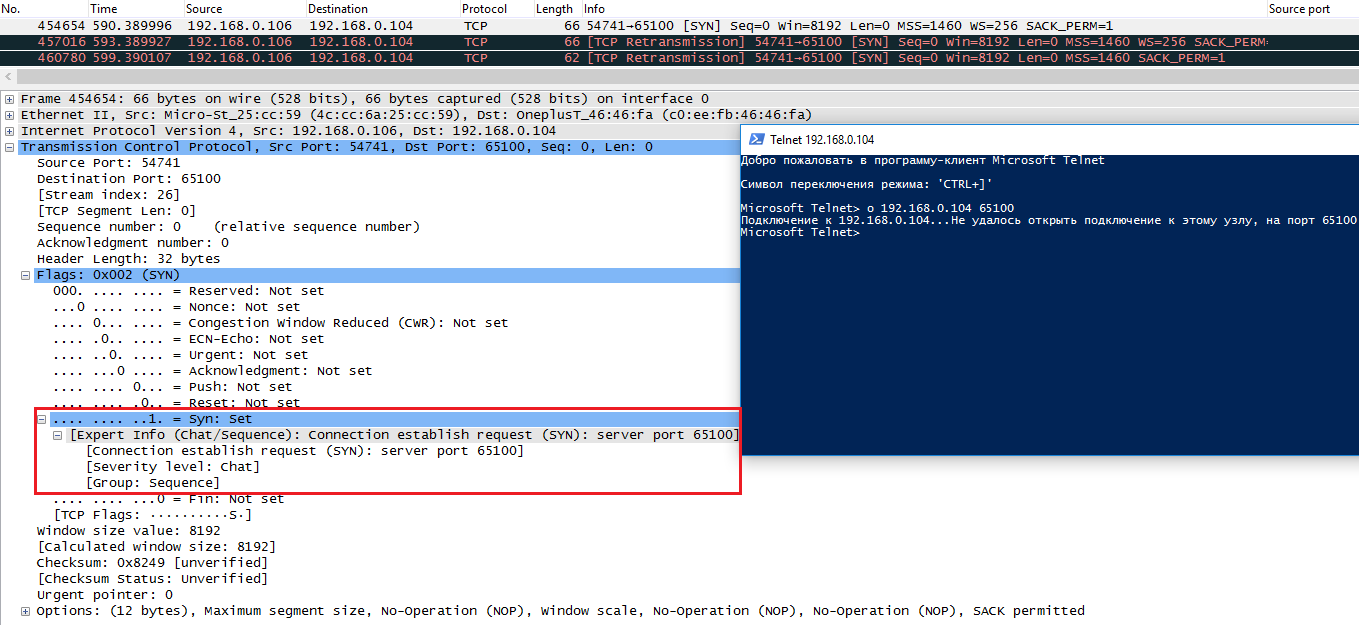
\includegraphics[scale = 0.50]{images/tcp6.png}
	
	\caption{Ожидание ответа на SYN}
	\label{image:20}
\end{figure}

Посылается несколько запросов на установление соединения с некоторым таймаутом, после чего клиент считает что хост недоступен. 

\section{Вывод}

В ходе работы был исследован сетевой трафик утилит ping и tracert а также протоколов ICMP, ARP и TCP.

На практике не имеет особого смысла исследовать трафик утилит ping и tracert, потому что они представляют полную и наглядную информацию о сетевом взаимодействии непосредственно внутри консоли. Однако, для выяснения причины ошибки соединения или для определения адресов и портов назначения исследование сетевого трафика подходит отлично.

Также необходимость анализа сетевого трафика обусловлена тем, что клиент-серверные приложения чаще всего не предоставляют полную информацию об используемом трафике. Анализаторы трафика по типу Wireshark имеют широкие возможности для фильтрации трафика, что позволяет просматривать сетевой трафик конкретных приложений. 

\clearpage

\section{Приложение 1}

\subsection{Установка соединения с закрытым портом при отключенном межсетевом экране}

Попробуем подключиться к закрытому порту компьютера с ОС Ubuntu по адресу 192.168.0.108:300 с компьютера с адресом 192.168.0.106. По умолчанию ОС Ubuntu имеет стандартный межсетевой экран ufw, который не позволяет узнать извне, какие порты открыты или закрыты (рис. 1.17). Для того, чтобы разрешить взаимодействие с портом 300 извне, воспользуемся утилитой iptables:

\begin{verbatim}
sudo iptables -I INPUT -p tcp --dport 300 -m state --state NEW -j ACCEPT
\end{verbatim}

Результат подключения к закрытому порту:

\begin{figure}[h!]
	\centering
	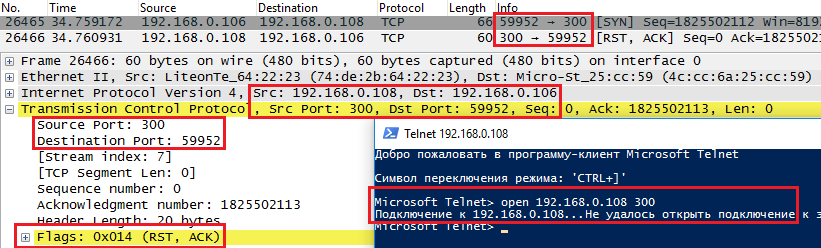
\includegraphics[scale = 0.80]{images/tcp7.png}
	
	\caption{Результат подключения к закрытому порту}
	\label{image:21}
\end{figure}

При попытке подключения к закрытому порту ожидаемо вернулся пакет с установленным флагом RST.

\end{document}